\setbeamercolor{background canvas}{bg=fitblue}
\begin{frame}
\frametitle{Tessellation / Teselace}
\begin{center}
\Huge {\color{white} Tessellation / Teselace}
\end{center}
\end{frame}
\setbeamercolor{background canvas}{bg=white}

\begin{frame}[fragile]
\frametitle{Tessellation / Teselace}
  \scriptsize
	\begin{itemize}
	\item Tessellation refines one primitive to multiple connected sub-primitives.
	\item The main purpose is to add geometric details.
	\item It is located before geometry shader and after vertex shader.
	\item It is composed of 3 parts: Control Shader, Primitive Generator/ Tessellator, Evaluation Shader.
	\item New type of primitive \textcolor{red}{GL\_PATCHES}
	\end{itemize}
	\begin{itemize}
	\item Teselace je rozřezání jednoho primitiva na více spojených.
	\item Může se použít pro zjemnění geometrie
	\item Nachází se za vertex shaderem a před geometry shaderem.
	\item Složená ze 3 částí: Contrl Shader, Generování primitiv/Teselace, Evaluation Shader
	\item Nový typ primitiva \textcolor{red}{GL\_PATCHES}
	\end{itemize}
  {\scriptsize
\begin{minted}[bgcolor=bg]{packages/c_cpp.py:CppLexer -x}
glPatchParameteri(GL_PATCH_VERTICES,10);//set the number of patch vertices
glDrawArrays(GL_PATCHES,0,100);//draw 10 patches each with 10 vertices
	\end{minted}
  }
	\begin{figure}[h]
	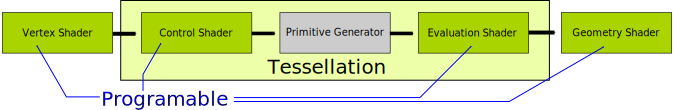
\includegraphics[width=10cm,keepaspectratio]{pics/tessellation/tess_pipeline.pdf}
	\end{figure}
\end{frame}

\begin{frame}
\frametitle{Control Shader}
  \scriptsize
	\begin{itemize}
	\item It controls the tessellation level.
	\item It computes control points.
	\item It is executed as many times as is the number of vertices in output patch.
	\item Vertex counting number is stored in \textcolor{OliveGreen}{gl\_InvocationID}
	\item \textcolor{OliveGreen}{barrier}()
	\end{itemize}

	\begin{itemize}
	\item Řídí stupěň teselace
	\item Počítá kontrolní body
	\item Je spouštěn tolikrát, kolik je vertexů ve výstupním primitivu
	\item Číslo spuštění uloženo v \textcolor{OliveGreen}{gl\_InvocationID}
	\item \textcolor{OliveGreen}{barrier}()
	\end{itemize}
	\begin{figure}[h]
	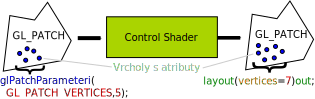
\includegraphics[width=10cm,keepaspectratio]{pics/tessellation/tess_control.pdf}
	\end{figure}
\end{frame}

\begin{frame}
    \frametitle{Tessellation levels, úrovně teselace}

    
\includegraphics[width=\textwidth]{pics/tessellation/tess.pdf}

    \begin{itemize}
				\item \textcolor{OliveGreen}{layout}
					(\{\textcolor{orange}{isolines},\textcolor{orange}{triangles},\textcolor{orange}{quads}\})
					\textcolor{OliveGreen}{in};
				\item \textcolor{OliveGreen}{gl\_TessLevelOuter}[4],\textcolor{OliveGreen}{gl\_TessLevelInner}[2]
    \end{itemize}
\end{frame}

\begin{frame}[fragile]
\frametitle{Control Shader - example}
	{\scriptsize
\begin{minted}[bgcolor=bg]{packages/graphics.py:GLShaderLexer -x}
#version 430

// the number of vertices in output patch
// the number of executions of control shader per input patch
layout(vertices=3)out;

uniform vec2 TessLevelInner;//inner tessellation
uniform vec4 TessLevelOuter;//outer tessellation

void main(){
  //the size of gl_in depends on GL_PATCH_VERTICES
  //the size of gl_out depends on layout(vertices=n)out;
  gl_out[gl_InvocationID].gl_Position=gl_in[gl_InvocationID].gl_Position;
  if(gl_InvocationID==0){
    gl_TessLevelOuter[0]=TessLevelOuter[0];
    gl_TessLevelOuter[1]=TessLevelOuter[1];
    gl_TessLevelOuter[2]=TessLevelOuter[2];
    gl_TessLevelOuter[3]=TessLevelOuter[3];
    gl_TessLevelInner[0]=TessLevelInner[0];
    gl_TessLevelInner[1]=TessLevelInner[1];
  }
}
	\end{minted}
	}
\end{frame}

\begin{frame}
\frametitle{Evaluation Shader}
  \scriptsize
	\begin{itemize}
		\item Selects primitive type \textcolor{Orange}{isolines},\textcolor{orange}{triangles},\textcolor{orange}{quads}.
		\item Computes location of vertices of tessellated primitive.
		\item Tessellation coordinates \textcolor{OliveGreen}{gl\_TessCoord}
		\item Generated primitives are sent to geometry shader.
	\end{itemize}
	\begin{itemize}
		\item Nastavuje typ primitiva \textcolor{Orange}{isolines},\textcolor{orange}{triangles},\textcolor{orange}{quads}
		\item Počítá souřadnice vrcholů nateselovaného primitiva
		\item Souřadnice do primitiva \textcolor{OliveGreen}{gl\_TessCoord}
		\item je spoštěn pro každý nateselovaný vrchol
		\item vygenerovaná primitiva jdou dále do geometry shaderu
	\end{itemize}
	\begin{figure}[h]
	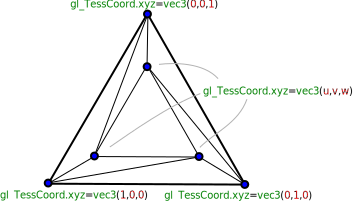
\includegraphics[width=7cm,keepaspectratio]{pics/tessellation/tess_coord.pdf}
	\end{figure}
\end{frame}


\begin{frame}[fragile]
\frametitle{Evaluation Shader - example}
  \scriptsize
	\begin{itemize}
		\item Tessellated quad
		\item Computation of new vertices using tessellation coordinates and control points.
	\end{itemize}
	\begin{itemize}
		\item Nateselovaný čtyřúhelník
		\item výpočet pozic vrcholů
	\end{itemize}
	{\scriptsize
\begin{minted}[bgcolor=bg]{packages/graphics.py:GLShaderLexer -x}
#version 430

layout(quads)in;

void main(){
  vec4 A=mix(gl_in[0].gl_Position,gl_in[1].gl_Position,gl_TessCoord.x);
  vec4 B=mix(gl_in[3].gl_Position,gl_in[2].gl_Position,gl_TessCoord.x);
  gl_Position=mix(A,B,gl_TessCoord.y);
}
	\end{minted}
	}
\end{frame}




\begin{frame}[fragile]
  \frametitle{Bézier surfaces - example}
	{\scriptsize
\begin{minted}[bgcolor=bg]{packages/graphics.py:GLShaderLexer -x}
// Vertex shader	
#version 430
void main() {
  gl_Position = mvp*position;
}

// Control shader
#version 430
layout(vertices=16) out;

void main() {
  gl_out[gl_InvocationID].gl_Position =
  gl_in[gl_InvocationID].gl_Position;
  if(gl_InvocationID == 0) {
    gl_TessLevelInner[0] = gl_TessLevelInner[1] = 
    gl_TessLevelOuter[0] = gl_TessLevelOuter[1] =
    gl_TessLevelOuter[2] = gl_TessLevelOuter[3] = 64;
  }
}
	\end{minted}
	}
\end{frame}

\begin{frame}[fragile]
    \frametitle{Bézier surfaces - example}
  	{\scriptsize
\begin{minted}[bgcolor=bg]{packages/graphics.py:GLShaderLexer -x}
// Evaluation shader
#version 430
layout(quads, ccw) in;

vec4 bernstein(float t) {
  return vec4((1-t)*(1-t)*(1-t), 3*t*(1-t)*(1-t), 3*t*t*(1-t), t*t*t);
}

void main() {
  vec4 bu = bernstein(gl_TessCoord.x);
  vec4 bv = bernstein(gl_TessCoord.y);
  vec4 position = vec4(0, 0, 0, 0);
  for(int y = 0; y < 4; ++y){
    for(int x = 0; x < 4; ++x){
      position += bu[x]*bv[y]*gl_in[4*y + x].gl_Position;
    }
  }
  gl_Position = position;
}
  	\end{minted}
		}
\end{frame}

\begin{frame}[fragile]
\frametitle{Shader Communication / Komunikace mezi shadery}
	{\tiny
\begin{minted}[bgcolor=bg]{packages/graphics.py:GLShaderLexer -x}
#version 430

//vertex shader
out vec4 vAttrib;
gl_Position

//control shader
//attrib from vertex shader. The array size is determined by glPatchParameteri(GL_PATCH_VERTICES,n);
in  vec4 vAttrib[];//atrib. from vertex shader
gl_in[].gl_Position;//position attribute from vertex shader
//output attribute from control shader to evaluation shader, the array size is determined by layout(vertices=n)out;
out vec4 cAttrib[];//atribut pro vrchol z control shaderu do evaluation shaderu
//per patch atribut z control shaderu do evaluation shaderu, pocet je 1
patch out mat4 cM;//atribut pro patch z control shaderu do evaluation shaderu

//evaluation shader
in vec4 cAttrib[];
patch in  mat4 cM;
//atribut z evaluation shaderu do geometry shaderu
out vec3 eNormal;

//geometry shader
//pocet je rizen typem primitiva
in vec3 eNormal[];
	\end{minted}
	}
\end{frame}

\begin{frame}[fragile]
    \frametitle{Příklad - Kružnice vepsaná}
  \begin{columns}[T]
    \begin{column}{.44\textwidth}
	    \begin{figure}[h]
    		\includegraphics[width=5cm,keepaspectratio]{pics/tessellation/ts_circle}
    	\end{figure}
    \end{column}
    \begin{column}{.48\textwidth}
 	    \begin{figure}[h]
    		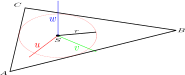
\includegraphics[width=5cm,keepaspectratio]{pics/tessellation/circle.pdf}
    	\end{figure}
{\tiny
$$
K=
\left( 
\begin{array}{cccc} 
1 & 0 & 0 & S_x \\
0 & 1 & 0 & S_y \\
0 & 0 & 1 & S_z \\
0 & 0 & 0 & 1  \\
\end{array}
\right)
\cdot
\left( 
\begin{array}{cccc} 
r & 0 & 0 & 0 \\
0 & r & 0 & 0 \\
0 & 0 & r & 0 \\
0 & 0 & 0 & 1  \\
\end{array}
\right)
\cdot$$
$$
\left( 
\begin{array}{cccc} 
u_x & v_x & w_x & 0 \\
u_y & v_y & w_y & 0 \\
u_z & v_z & w_z & 0 \\
0 & 0 & 0 & 1  \\
\end{array}
\right)
$$
}
    \end{column}
  \end{columns}
\end{frame}

\begin{frame}[fragile]
    \frametitle{Příklad - Kružnice vepsaná}
  \begin{columns}[T]
    \begin{column}{.44\textwidth}
      Control Shader
  	{\tiny
\begin{minted}[bgcolor=bg]{packages/graphics.py:GLShaderLexer -x}
#version 400
layout(vertices=1)out;
patch out mat4 K;
void main(){
  gl_TessLevelOuter[0]=1;
  gl_TessLevelOuter[1]=64;
  gl_TessLevelOuter[2]=1;
  gl_TessLevelOuter[3]=1;
  gl_TessLevelInner[0]=1;
  gl_TessLevelInner[1]=1;
  vec4 TT[3];
  TT[0]=gl_in[0].gl_Position;
  TT[1]=gl_in[1].gl_Position;
  TT[2]=gl_in[2].gl_Position;
  float t01=length((TT[0]-TT[1]).xyz);
  float t02=length((TT[0]-TT[2]).xyz);
  float t12=length((TT[1]-TT[2]).xyz);
  float s=t01+t02+t12;
  float r=sqrt((s/2-t01)*(s/2-t02)*(s/2-t12)*s/2)*2/s;
  t01/=s;
  t02/=s;
  t12/=s;
  vec3 C=TT[0].xyz*t12+TT[1].xyz*t02+TT[2].xyz*t01;
  vec3 x=normalize(TT[0].xyz-C);
  vec3 y=normalize(TT[1].xyz-C);
  vec3 z=normalize(cross(x,y));
  y=normalize(cross(z,x));
  K=mat4(vec4(x,0)*r,vec4(y,0)*r,vec4(z,0)*r,vec4(C,1));
}
  	\end{minted}
		}
    \end{column}
    \begin{column}{.48\textwidth}
      Evaluation Shader
  	{\tiny
\begin{minted}[bgcolor=bg]{packages/graphics.py:GLShaderLexer -x}
#version 400

#define MY_PI 3.14159265359

layout(isolines)in;

uniform mat4 V;
uniform mat4 P;

patch in mat4 K;

void main(){
  float Angle=gl_TessCoord.x*MY_PI*2;
  vec4 PP=vec4(cos(Angle),sin(Angle),0,1);
  gl_Position=P*V*K*PP;
}
  	\end{minted}
		}
    \end{column}
  \end{columns}

\end{frame}


\begin{frame}
\frametitle{Jak moc teselovat?}
	Outer level:
	\begin{itemize}
	\item Strany ploch musí odpovídat (zamezení T-spojů)
	\item Transformovat kontrolní body na obrazovku
	\item Spočítat delků hran
	\item Dělit maximální delkou hrany
	\end{itemize}
	Inner level:
	\begin{itemize}
	\item Z přílušných outer-levelů
	\item průměr, maximum, ...
	\item Korekce podle vnitřních kontrolních bodů
	\end{itemize}
	Ukázka v aplikaci
\end{frame}

